\section{Methodology}

\subsection{Theory}
\begin{marginfigure}
    \begin{tikzpicture}
    \node[obs]                (x) {\(\x\)};
    \node[latent, left=of x]  (z) {\(\z\)};

    \edge {z} {x} ; %

    \plate {xz} {(x)(z)} {\(N\)} ;
\end{tikzpicture}
%
    \caption{The used graphical model for the source separation task. We have the latent source channel variables. Exemplary here, as in our data, we have four sources. The mix \(\B{m}\) is observed.}%
    \label{fig:graphical_model}
\end{marginfigure}

We propose the graphical model as shown in \cref{fig:graphical_model} as the generative story of the source separated music tracks. For each source is sampled from the latent source distribution. The observed mix is generated deterministically from the full set of sources, which is a known function of the sources samples. Without loss of generality we fix this function to be the mean.

\begin{fullwidth}
    \newcommand{\ppost}{{q_{\B{\φ}_k}(\B{s}_k|\B{m})}}
    \newcommand{\post}{p(\B{s}_1,\…,\B{s}_N|\B{m})}
    \begin{align}
        \log p_{\B{\θ}}(\B{m})
        &= \idotsint \log p(\B{m}) \· \Π_k^N \ppost \,d^N \B{s}\\
        &= \E_\ppost^N \left[ \log p(\B{m}) \right]\\
        &= \E_\ppost^N \left[ \log \÷{p(\B{m},\B{s}_1,\…,\B{s}_N)}{\post} \right]\\
        &= \E_\ppost^N \left[ \log \÷{p(\B{m}|\B{s}_1,\…,\B{s}_N) \· \Π_k^N p(\B{s}_k)}{\Π_k^N \ppost} + \log \÷{\Π_k^N \ppost}{\post} \right]\\
        &\geq \Σ_k^N \E_\ppost \left[ \log \÷{p(\B{s}_k)}{\ppost} \right]
             +\E_\ppost \left[ p(\B{m}|\B{s}_1,\…,\B{s}_N) \right]\\
    \end{align}
\end{fullwidth}

Big assumption here \(p(\B{m},\B{s}_1,\…,\B{s}_N) \equiv p(\B{m}|\B{s}_1,\…,\B{s}_N) \· \Π_k^N p(\B{s}_k)\)

\subsection{Datasets}
\subsection{ToyData}
\begin{marginfigure}
    \resizebox{\textwidth}{!}{%
        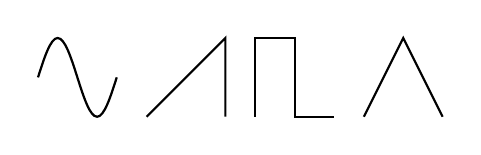
\begin{tikzpicture}
    \node[matrix,thick,column sep=1em,row sep=1em]
    {
        \draw (0,0.5) sin (0.25,1) cos (0.5,0.5) sin (0.75,0) cos (1,0.5); &
        \draw (0,0) -- (1,1) -- (1,0); &
        \draw (0,0) -- (0,1) -- (0.5,1) -- (0.5,0) -- (1,0); &
        \draw (0,0) -- (0.5,1) -- (1,0); \\
    };
\end{tikzpicture}
%
    }%
    \caption{One period of each of the four toy sources: sinus, sawtooth, square and triangle wave.}%
    \label{fig:toy_data}
\end{marginfigure}

We simplify the problem domain to create a toy-like dataset. We randomly generate waves from four simple oscillations, see~\cref{fig:toy_data}. Given a wave from each source, the mix is computed by simply taking the mean. When sampling from each source we randomly select a period and phase. The frequencies are restricted to the frequency bounds of the 88 keys of a equal-temprament tuned piano. In our experiments we are gonna model these sources with probability density, looking especially at the square that will pose a problem, as those only consist of two unique values (\(-1\) and \(1\)). This collapsing posterior would simplify the problem too much, therefore we also vary the amplitude of the sampled signals.

In ++later++ section we show that estimating densities over these waves is not giving a smooth manifold. Or differently: in the latent space we can not interpolate between two signals, because the model models, simply put, the sample waves as spiked Dirac deltas.


\subsection{musdb18}
Further we use the \emph{musdb18}~\cite{rafiiMUSDB182017} dataset published for the 2018 Signal Separation Evaluation Campaign~\cite{stoter20182018}. The datasets consits of 150 full songs covering various artists and genres, splitted into train and test sets sized 100 and 50, respectively. Each track is separated into the four sources \emph{drums}, \emph{bass}, \emph{vocals} and \emph{others}. The \emph{others} source channel contains any set of instrument not categorized under the first three ones. The song files are provided in the Stem audio file format~\cite{nativeinstrumentsStem} and encoded at 44.1kHz. Stem here is terming the provided source channels, we use the terms interchangeably.

Next to the separated stems, the dataset provides the original (studio) mix for each song. This mix is not equivalent to the simple linear mixing which we get by taking the mean. Nevertheless the provided mix diverges only insignificantly from a auto-generated mix, as the original sources are provided in their post-compression, post-mixed form. This means that we can use the original mix and assume it to be reasonably close to the kanonical linear mix.

As the songs are real natural songs, they are of different lengths. Our models will, in difference to many other recent methods, not be auto-regressive. Thus we sample fixed-length cuts from the songs as training and test samples. For the musdb data no pre-processing is applied, as the data already contains the wanted level variability, it spanning different genres and artists.

It is noted that the musdb18 dataset, while providing a remarkable diverse 10hr of real-world music, is a rather small numbered set of samples. Any data modeling from this set of data will consequently be biased. The dataset specifically is created for the accompying separation challenge and will not translate to general music modeling.
